\documentclass[a4paper,12pt]{article}
\usepackage[latin1]{inputenc}
\usepackage[spanish]{babel}
\usepackage{bm}
\usepackage{graphicx}
\usepackage{amsmath}
\setlength{\textheight}{235mm}
\setlength{\textwidth}{168mm}
\setlength{\oddsidemargin}{0pt}
\pagestyle{empty}
\begin{document}
\mbox{}\vspace*{-45mm}

{\centering
{\small\sc Escuela T�cnica Superior de Ingenieros de Caminos, Canales y
Puertos (Madrid)}\\*[4mm]
{\Large\bf M�todo de los Elementos Finitos 22-23}\\*[4mm]
Puntuable 2: Ecuaci�n de difusi�n \\*[4mm]
}

\vspace{3mm}

%%%%%
\noindent
La figura muestra la secci�n transversal de un r�o canalizado (de $1$ m de espesor), limitado por dos pantallas impermeables. En el interior, se encuentra un dique impermeable cimentado sobre un suelo 2. La geometr�a del r�o, dique, pantallas, suelo 1 y 2 se muestra en la figura debajo. 

En la zona derecha inferior se ha dejado abierto un espacio, de $1$ m de altura, sometido a la presi�n atmosf�rica.

El suelo 1 tiene un coeficiente de permeabilidad $k=10^{-3}$ m/s y est� por encima de un terreno impermeable. El suelo 2 tiene un coeficiente de permeabilidad $k=3 \cdot 10^{-3}$ m/s.

Para analizar las filtraciones que se producen se realizar� un modelo plano de elementos finitos que represente dicha secci�n transversal. La discretizaci�n a efectuar corresponde a elementos cuadrados de cuatro nodos de lado $0.30$ m. Considerar la opci�n de forma de elemento Quad Dominated, y con t�cnica tipo Free. 

{\bf NOTA: Para homogeneizar los valores de la altura piezom�trica se tomar� como altura geom�trica $z=0$ la de los puntos del terreno impermeable}

\begin{center}
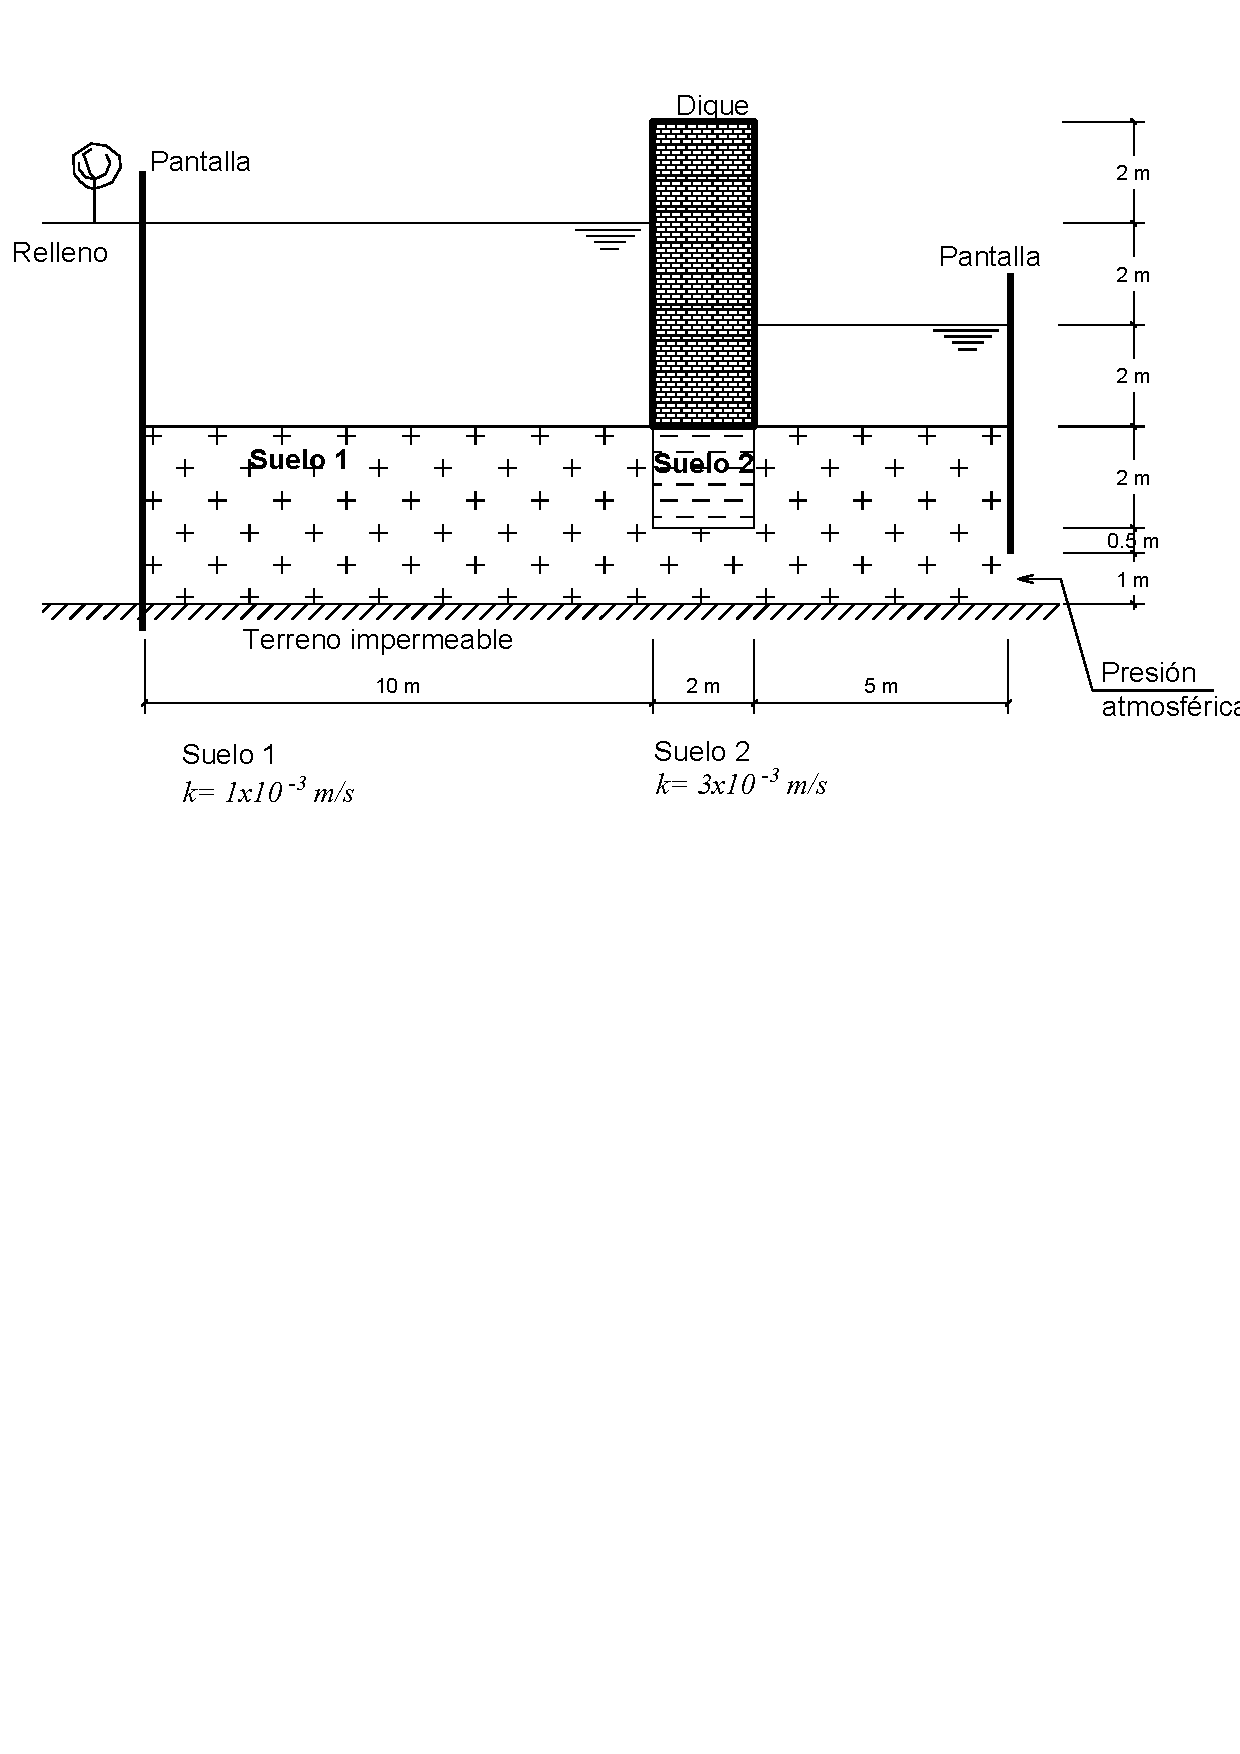
\includegraphics[width=0.7\textwidth]{ejerc2}
\end{center}

\end{document}
